\documentclass{sig-alternate}
\usepackage{url}
\usepackage{graphicx}
\usepackage{subfigure}
\usepackage{url}

\begin{document}

\newcommand{\todo}[1]{\textbf{TODO}\footnote{\textbf{TODO:} #1}}


\title{An exploration of the pull-based software development model}
\numberofauthors{3}

\author{
\alignauthor
Georgios Gousios\\
       \affaddr{Delft University of Technology}\\
       \affaddr{Delft, The Netherlands}\\
       \email{G.Gousios@tudelft.nl}
\alignauthor
Martin Pinzger\\
       \affaddr{Delft University of Technology}\\
       \affaddr{Delft, The Netherlands}\\
       \email{M.Pinzger@tudelft.nl}
\alignauthor
Arie van Deursen\\
       \affaddr{Delft University of Technology}\\
       \affaddr{Delft, The Netherlands}\\       
       \email{Arie.vandeursen@tudelft.nl}
}

\maketitle

\begin{abstract}

  The advent of distributed version control systems has led to the development
  of a new paradigm for distributed software development; instead of pushing
  changes to a central repository, developers pull them from other repositories
  and merge them locally. Various code hosting sites, notably Github, have
  tapped on the opportunity to facilitate pull based development by offering
  workflow support tools, such as code reviewing systems and integrated issue
  trackers. In this work, we provide an exploration of how pull-based software
  development works. By quantitatively analysing a hundred projects, we
  identify the factors that affect pull request processing speed and
  create a classifier able of predicting whether pull requests will be accepted
  with 85\% accuracy.  

\end{abstract}

% A category with the (minimum) three required fields
\category{H.4}{Information Systems Applications}{Miscellaneous}
%A category including the fourth, optional field follows...
\category{D.2.8}{Software Engineering}{Metrics}[complexity measures, performance measures]

\terms{Theory}

\keywords{pull-based development, pull request, collaborative development}

\section{Introduction}

Since their appearance in 2001, distributed version control systems ({\sc
dvcs}), notably Git, have revolutionized the way distributed software
development is carried out. Driven by pragmatic needs, {\sc dvs}s were designed
from scratch to work as an advanced patch management systems, rather than a
versioned file system, the then dominant version control system ({\sc vcs})
paradigm. In most {\sc dvcs}s, a file is an ordered set of changes, the serial
application of which lead to the current file, and consequently file tree,
state. The changesets can originate from a local filesystem or a remote host;
tools facilitate the acquisition and application of changesets on a local
mirror. The distributed nature of {\sc dvcs}) enables a pull-based development
model, where changes are offered to a project repository through a network of
project forks; it is up to the repository owner to accept or reject the incoming
pull requests.

Several code hosting sites, including Github and BitBucket, tapped on the
opportunity to make the pull-based development model more accessible to
programmers. A unique characteristic of such sites is that they allow any user
to fork any public repository. The clone creates a public project that belongs
to user that cloned it, so the user can modify the repository without being part
of the development team. What is more important is they automate the selective
contribution of commits from the clone to the source, through pull requests. As
mentioned earlier, pull requests are not unique to code hosting sites; in fact,
the Git software distribution includes the \textsf{git-request-pull} utility
which provides the same functionality at the command line. Github
improved\footnote{Not everyone agrees:
\url{https://github.com/torvalds/linux/pull/17}} this process significantly by
integrating code reviews, discussions and issues, thus effectively lowering the
entry barrier for casual contributions. Combined, cloning and pull requests
create a new development model, where changes are pushed to the project
maintainers and go through code review by the community before being integrated. 

Pull-based development is an emerging paradigm for distributed software
development. As more developers appreciate the perceived benefits of isolated
development and branching~\cite{Bird12}, more projects, both closed source and,
especially, open source are being migrated to code hosting sites with support
for pull based development~\cite{Barr12}. Our work investigates the following
research questions:

\begin{description}
  
  \item[RQ1] How widespread is the use of the pull-based development model? What
    are its characteristics?
  
  \item[RQ2] What are the factors that affect the decision to merge of a pull request?

  \item[RQ3] Can we predict whether a pull request will be merged to a
    repository?

\end{description}

To answer the above questions, we conducted a quantitative exploration of the
way the pull-based distributed software development model works.
Our study is based on data from the Github
collaborative development forge, as made available through the GHTorrent
project~\cite{GS12}. Specifically, we used a dataset slice that covered activity
across all projects on Github from early February 2012 to early Feb 2013.
Github offers two types of data through its {\sc api}; a streaming data flow
listing events, such as forking or creating pull requests, happening on
repositories and a static view of entity states. To obtain references to the
roots of the static view entities, the event stream needs to be followed. From
there, a recursive dependency-based parsing approach can yield all data
offered through the {\sc api}. 
The GHTorrent dataset covers a broad range of development activities on Github,
including pull requests and issues. On Feb 2013, more than a million 
pull requests from more that a hundred thousand projects have been collected by the project.

Using the GHTorrent dataset, we explore the use of pull requests among projects
in Github to answer {\sc rq1}. Based on our observations, we develop a theory
of pull request adoption.
To answer {\sc rq2} and {\sc rq3}, we examined a hand selected group of 50 Ruby, Java and Scala projects,
(\todo{Add number of pullreqs} pull requests), and identified, using machine
learning tools, common factors that affect pull request lifetime and merging. We
then applied the extracted models on another group of 50 randomly selected
projects in order to validate them. The results show that it is
possible to predict, with a high accuracy, whether a pull request will be
merged.

In the following section, we briefly describe the pull-based development model
and present an overview of how pull based development works on Github.
Then, we examine pull requests from various view points and develop
a theory of how pull requests are processed. In Section~\ref{sec:accrej},
we test the developed theory against statistical models and discuss our
findings in Section~\ref{sec:discussion}.

\section{Pull-based development}

\subsection{Development models with DVCs}

The development models afforded by {\sc dvcs}s are a superset of 
those in centralized version control environments~\cite{Shiha12,Bird09}. 
With respect to receiving and processing external contributions,
the following strategies can be employed:

\begin{description}

  \item[Shared repository] Developers share a common repository, with read and
    write permissions. To work, they clone it locally, modify its contents,
    potentially introducing new branches, and push their changes back to the
    central one. To cope with multiple versions and multiple developers, larger
    projects usually adopt a {\em branching model}, i.e. an organized way to
    accept and test contributions before those are merged to the main
    development branch~\cite{Bird12}. While the exact details depend on the
    project requirements, usually branching models include feature branches,
    where developers implement new features and fix bugs, and release branches,
    which store the state of each project release. After the work has finished
    on the feature branch its contents are merged appropriately to release
    branches and the project master branch.

  \item[Pull requests] The project repository is not shared among developers;
    instead, developers clone the repository and make their changes independent
    of each other. When a set of changes is ready to be submitted with the main
    repository, they create a pull request, which specifies a branch and a list
    of commits to merge with a branch in the main repository. The main
    repository owner is responsible to test the changes and pull them to the
    project's master branch. On larger projects, such as the Linux kernel,
    there are several layers of merge repositories before a contributed 
    pull request reaches the main tree~\cite{Cornf10}.

  \item[Intra-branch pull requests] As pull requests only specify branches from
    which certain commits can be pulled, there is nothing that forbids their use
    in the shared repository approach. In such cases, developers specify as the
    source a branch in the same repository as the target one.
    Intra-branch pull requests are usually accompanied by code reviews and
    discussion; this is why they are primarily performed if the project tooling
    supports this kind of interaction.

\end{description}

The use of branches in the shared repository model has been found to allow
developers to collaborate on tasks in highly cohesive branches, while enjoying
reduced interference from developers working on other tasks, even if those tasks
are strongly coupled to theirs~\cite{Barr12}. On the other hand, non-frugal
use of branching can lead to measurable, but not significant, delays in 
projects~\cite{Bird12}. In this work, we only consider pull-based development
as our investigation target.

\subsection{Pull-based development on Github}

Github is a very popular development site; in in its main page, Github reports
more than 5 million repositories and 3 million users. However,  not all those
projects are active: in 2012, the GHTorrent dataset captured events initiated by
(approximately) 1,260,000 users affecting 2,088,000 repositories. The majority
of registered repositories are forks of other repositories, special repositories
hosting user web pages (named as \texttt{<name>.github.com}), program
configuration files (\texttt{dotfiles}) and temporary repositories for
evaluating Git (\texttt{try\_git}). In the GHTorrent dataset, less than half
(905,400 or 42\%) of the active repositories are original repositories. From
those, only 587,800 (or 28\% in total) received a commit in 2012.

Github supports all types of distributed development outlined above; however,
pull requests receive special treatment. The site is tuned to allow easy forking
of projects by external users, while automating the generation of pull
requests through automatic comparison of project branches. In common to
Git-based pull requests, a Github pull request contains a list of commits
to be merged. In addition, the list of commits is automatically updated when newer commits have been added to the forked repository after the pull request
has been created. Each Github pull request has an attached implicit state
machine (see Figure~\ref{fig:state}), which is automatically updated by
Github as users manipulate the pull request.

\begin{figure}
  \begin{center}
    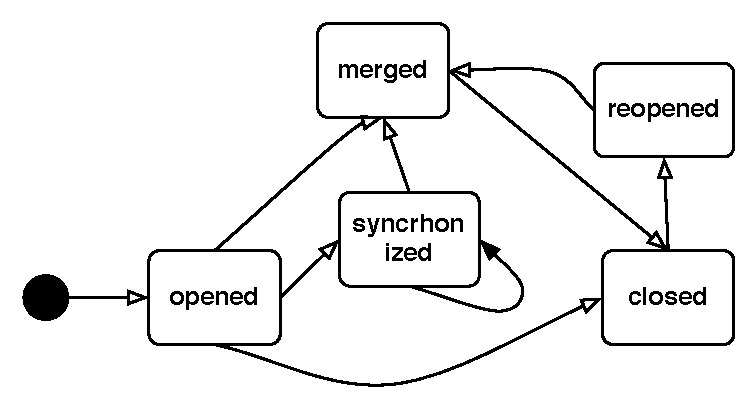
\includegraphics[scale=0.5]{pr-state-machine.pdf}
  \end{center}
  \caption{States into which a Github pull request can be into}
  \label{fig:state}
\end{figure}

By default, pull requests are submitted to the base repository for review.
Reviews can either target the pull as whole or the individual commits,
thereby resembling a code review. 
Even though any Github user can participate to the
review process, usually it is project community members that do so:
only 0.011\% of pull request comments come from users that have not
committed to the project repository.
Pull requests receive comments quite frequently: on average, each pull
request receives 12 (quantiles: 5\%: 2, 95\%: 35) discussion comments.

As a result of the discussion, pull requests can be updated with new commits or
be closed as redundant or uninteresting. To merge a pull request, a user must
be part of the main project team. The versatility of the Git tool suite enables
pull requests to be merged in various ways, presented below ordered by
the amount of preservation of the original source code properties:

\begin{description}

  \item[Through Github facilities] Github can automatically verify whether a
    pull request can be merged without conflicts to the base repository. When a
    merge is requested, Github will automatically apply the commits in the pull
    request and record the merge event. All authorship and history information
    is maintained in the merged commits.

  \item[Git merge] When a pull request cannot be applied cleanly or when
    project-related policies do not permit automatic merging, a pull request
    can be merged using plain Git utilities, using the following
    techniques: 

    \begin{itemize}

      \item \emph{Branch merging:} The remote branch containing the pull
        request commits is added as a source to a local repository. The remote 
        branch is merged to a local upstream branch, which is then pushed to
        the central repository or published for further pulling by other
        developers. Both history and authorship information are maintained,
        but Github cannot detect the merge in order to record a merge. 

      \item \emph{Cherry-picking:} Instead of merging all commits, the merger
        picks specific commits from the remote branch, which then applies to the
        upstream branch. The commit unique identifier changes, so exact history
        cannot be maintained, but authorship is preserved.
    
    \end{itemize}

    A technique that complements both of the above is \emph{commit
    squashing}: when the full history is not of interest to the project,
    several consecutive commits are merged into a single one on the pull request
    branch, which can them be merged or cherry-picked to the upstream branch. In
    this case, the author of the commit is different from the person that
    applied the commit.

  \item [Committing the patch] Through this technique, the merger creates a
    textual difference between the upstream and the pull request branch, which
    then applies to the upstream branch. Both history and authorship information
    is lost.

\end{description}

Pull requests are enabled by default on all repositories opened on Github.  From
the set of original repositories as described above, 88.000 (or 14\%) received
at least one pull request in 2012.  While the mean number of pull requests per
project is relatively low at 6.5 (percentiles: 5\%: 2, 95\%: 19), the
distribution of pull requests in projects is highly skewed, as shown in
Figure~\ref{fig:prfreq}.  A few large projects (such as the Homebrew package
manager and the Ruby on Rails web application framework) receive the vast
majority of pull requests. From the pull requests that have been opened in
2012, 60,45\% have been merged, thereby indicating that pull requests in
principle can work as a medium for obtaining external contributions.  Moreover,
even though one might expect that it is the well known projects that receive
most pull requests, this is not supported by our data: the Kendall rank
correlation between the number of watchers of a project and the number of pull
requests it has received is 0.32 ($p < 0.001, n = 63335$).

\begin{figure}
  \begin{center}
    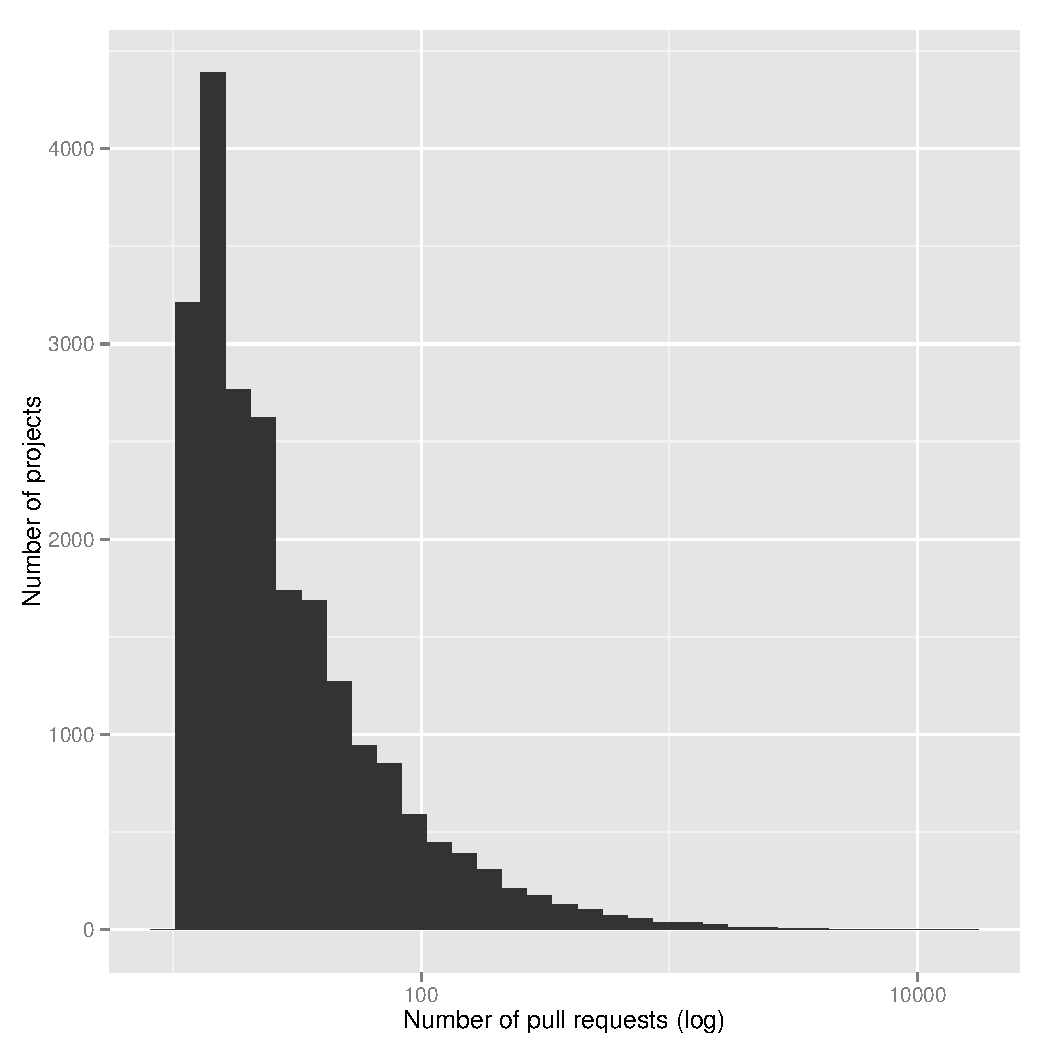
\includegraphics[scale=0.4]{pull-req-freq}
  \end{center}
  \caption{Histogram of pull request frequencies for projects with more than
  10 pull requests.}
  \label{fig:prfreq}
\end{figure}

Issues and pull requests are dual on Github; for each pull request, an
issue is opened automatically. Commits can also be attached to issues to
convert them to pull requests (albeit with external tools). This duality
enables project administrators to treat pull requests as work items,
which can be managed using the same facilities used for issues.
Across projects that received pull requests in 2012, 

A phenomenon related to pull requests is ``drive-by'' pull requests. As the
relative cost to fork a repository is negligible on Github (54\% of the
repositories are forks), it is not uncommon for developers to fork other
repositories to perform casual commits, such as fixes to spelling mistakes or
indentation issues~\cite{Pham13}. In addition, Github provides web based editors
for various file formats, using which any user can edit a file in another
repository; behind the scenes, Github will fork the repository and ask the user
to create a pull request to the original one. Such commits might be identified
as pull requests that contain a single commit from users that are not yet part
of the project's community. Even under this na\"ive definition, 7\% of pull
requests in 2012 can be classified as drive by commits. Moreover, 3.5\% of the
forks were created for the sole purpose of creating a drive-by commit.  More
work needs to be done for the accurate definition and assessment of the
implications of drive-by commits, which we defer for future work.

Pull requests are an important medium for collaborative software development.

\begin{figure}
  \begin{center}
    
\includegraphics[scale=0.5]{num-commiters-after-pr}
  \end{center}
  \caption{Number of committers before and after the introduction of pull
  requests by Github. The lines are smoothed using the local polynomial
  regression fitting method, to omit minor monthly fluctuations.}
  \label{fig:}
\end{figure}

\section{Collaboration through pull requests}

Software development can be distributed across various dimensions~\cite{Gumm06};
among them, physical distribution distributes programming tasks across people
collaborating remotely, while temporal distribution distributes tasks to people
working in different time zones. Distribution of development activities has been
initially thought to hinder collaboration~\cite{Herbs99, Batti01}, even though
subsequent studies have shown that it does not pose significant threats to
project quality~\cite{Spine06, Nguye08, Bird09a}. Access to online collaboration
tools such as {\sc vcs} and bug databases have been identified as a necessary
requirement for collaborative software development~\cite{Knuds76,Pilat06,
Catal06}. Distributed collaboration on software artifacts can be facilitated
through awareness building tools: 

We advocate that pull requests as a distributed development model in general,
and as are implemented by Github in particular, form a new method of
collaboration for distributed software development. The novelty lays on
the decoupling of the development effort from the decision to incorporate
the results of the development in the code base. 
By separating the concerns of building artifacts and incorporating
changes, work is cleanly distributed among a core team which is responsible
to perform the merges and a peripheral team that submits, often occasional,
changes to be considered for merging. 
The review mechanism that Github incorporates has the additional effect of
improving awareness~\cite{Dabbi12}; core team developers can 

A question that emerges is what are the factors that affect the efficiency
of the collaboration in pull-based development. Intuitively, a pull request
based collaboration is effective when the suitability of the pull request for
a project can be assessed and merged (or rejected) fast. 

Based on prior work~\cite{Weiss08}, we expect small pull requests to be easier to accept that larger ones. Similarly, pull requests that affect an active
area of the project would be easier to process~\todo{ref?}
In reference ~\cite{Bird07}, Bird et al. presented evidence that social
reputation has an impact on whether a


\section{Data Preparation}

In the previous section, we defined pull based development, and presented an
overview of how it works across all projects on Github. While an overview of the
activity in 2012 can be safely extracted from the dataset, several limitations
would not allow us to apply our detailed analysis across all projects.
Specifically, due to the incremental nature of the GHTorrent dataset collection,
only data that are linked from events (and their dependencies) are being
collected. Projects worth analyzing have a history longer than a year, so it is
important to retrieve all information available during the project's life. To
make the data collection, and subsequent analysis, practical, we restricted our
input data to two datasets, a \textsf{handpicked} and a \textsf{random} one. 
Both datasets contain 50 projects of different sizes each. The 
\textsf{handpicked} dataset was 


To build the datasets, we set forth the following requirements when selecting
projects to include:

\begin{itemize}

  \item Adequate number of pull requests. For the \textsf{handpicked} dataset,
    we wanted to 

  \item Projects should include tests. To measure the effect of testing on pull
    request acceptance, we could only use projects that include tests which we
    could measure reliably. For that, we exploited the convention-based project
    layout in the Ruby (Gem), Java and Scala (both Maven) language ecosystems,
    so our project selection was limited to those languages. 

  \item 

\end{itemize}

The \textsf{handpicked} dataset was constructed by manually browsing Github
and selecting projects with the above characteristics.  

\section{Characteristics of pull requests}
In this section, we focus on the characteristics of pull requests. 

\subsection{Lifetime of pull requests}

\begin{figure*}
\centering
\subfigure[Percentage of pull requests that have been merged before being closed]{
  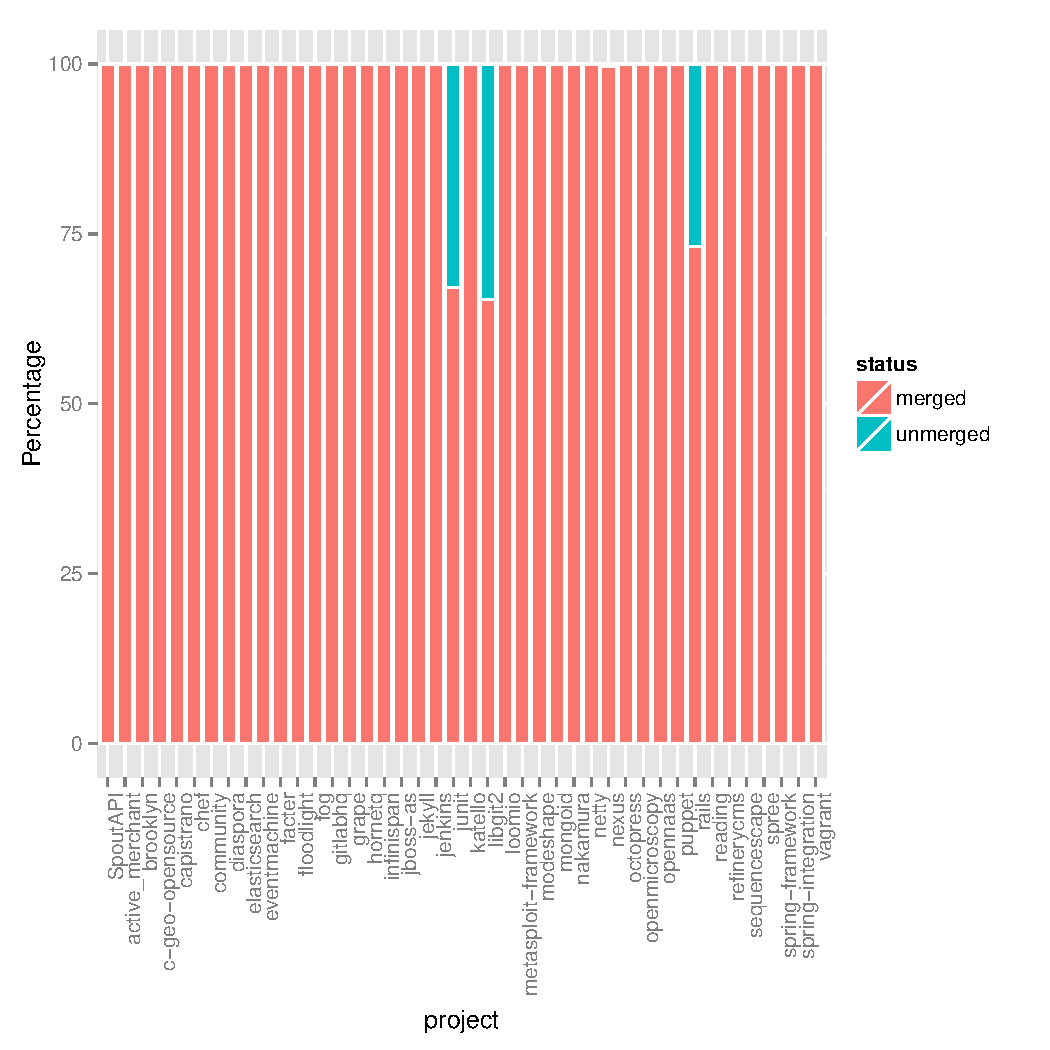
\includegraphics[scale=0.4]{perc-merged.pdf} 
  \label{fig:perc-merged}
}
\subfigure[Frequency distribution of lifetime for merged pull requests]{
%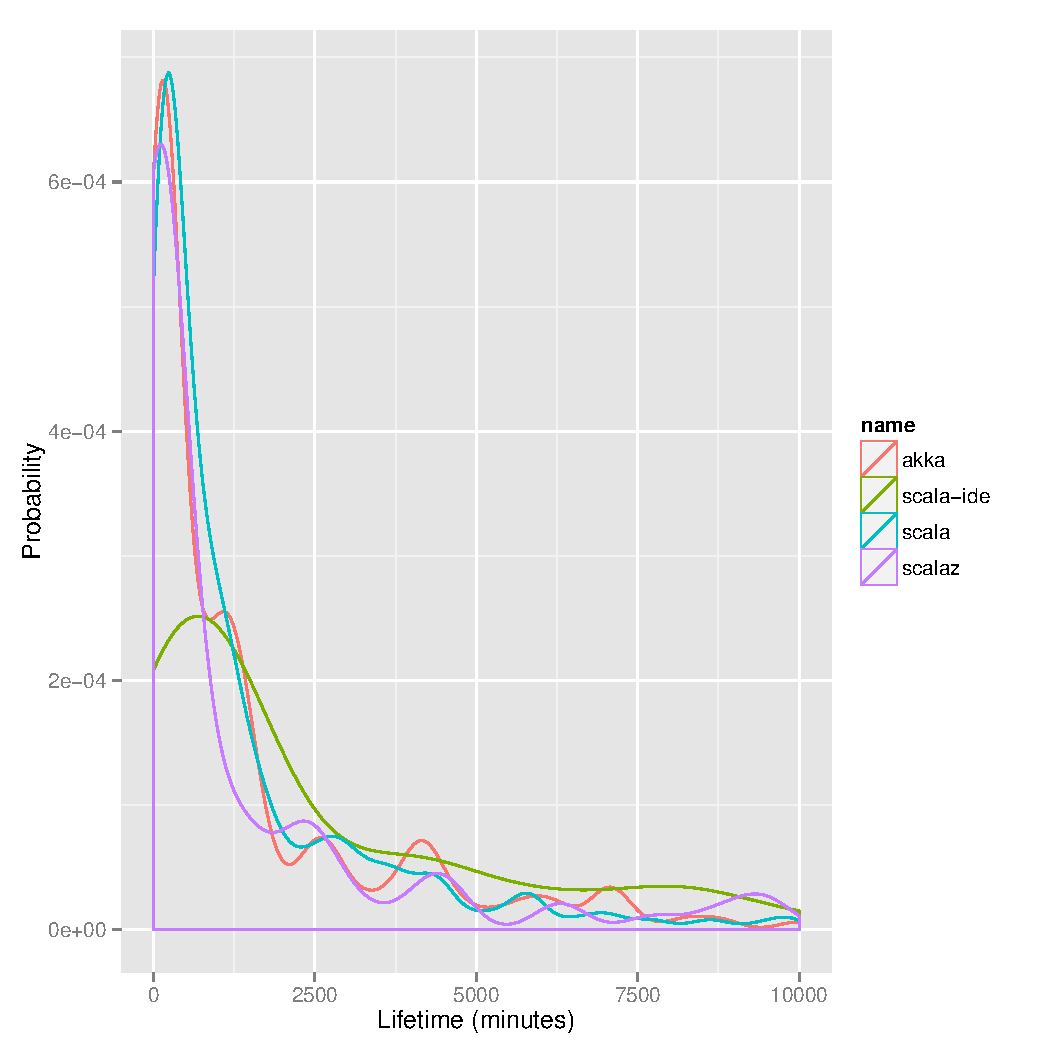
\includegraphics[scale=0.3]{lifetime-freq.pdf}
\label{fig:lifetime-freq}
}
\subfigure[Lifetime statistics for merged pull requests]{
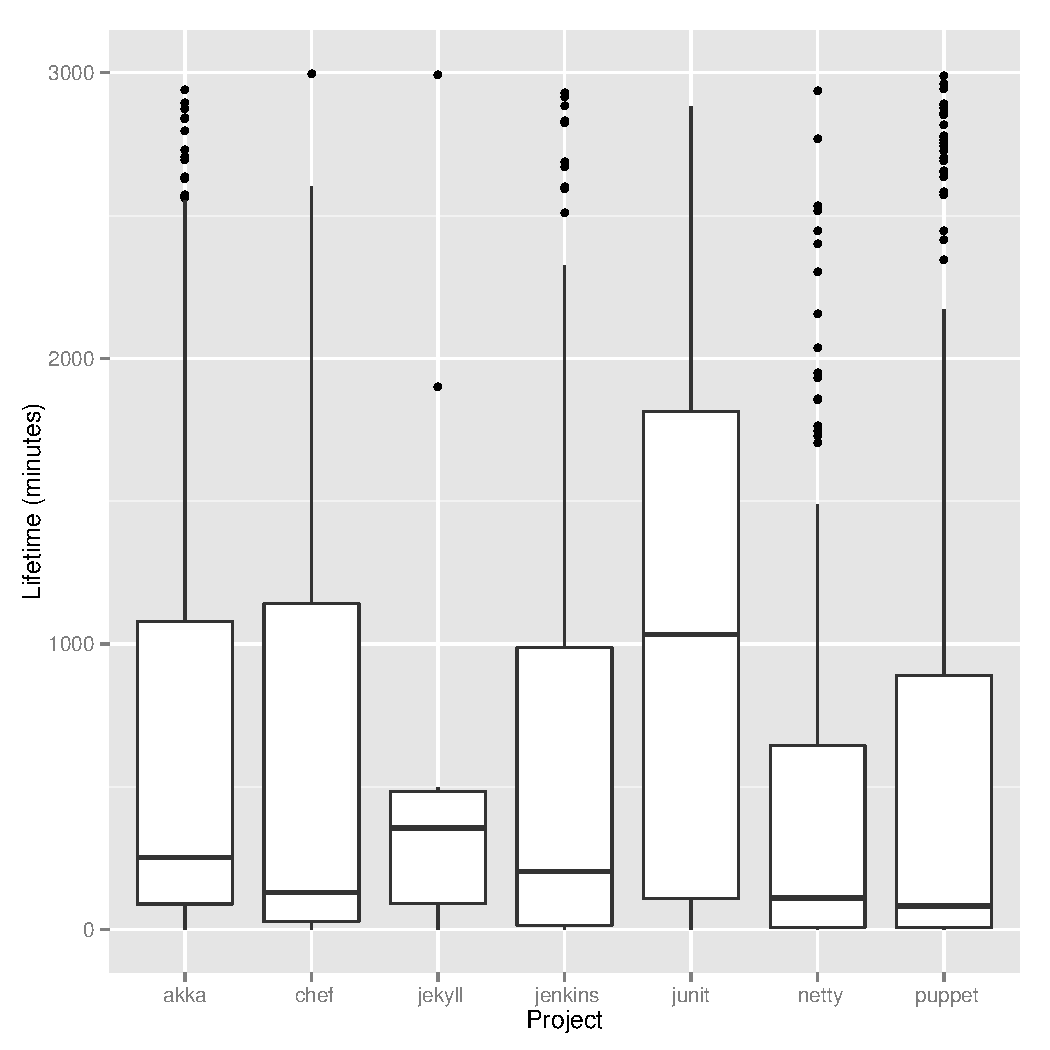
\includegraphics[scale=0.3]{lifetime-boxplot.pdf}
\label{fig:lifetime-boxplot}
}
\caption{Plots of pull request life time.}
\end{figure*}


An important observation is that there are several pull requests whose
lifetime is only limited to a ver

\subsection{Sizes of pull requests}


\subsection{Discussion and Code review}

Once a pull request has been submitted, it is open for discussion. 

\subsection{Team size}

\subsection{Testing}

\section{Acceptance and rejection}
\label{sec:accrej}

\begin{table*}
  \begin{small}
  \centering
  \begin{tabular}{rp{25em}}
    \hline
    \bf{Feature} & \bf{Description and Justification}\\
    \hline
    \multicolumn{2}{l}{\bf{Pull Request Impact}}\\
    
    \texttt{num\_commits} & Number of commits in the pull request. A bigger
    pull request will be slower to examine and therefore to merge.\\
    
    \texttt{churn} & Number of lines changed (added + deleted) by the pull request. The more lines changed, the longer a pull request will take to be
    reviewed.\\

    \texttt{files\_changed} & Number of files touched by the pull request. An
    indication of the impact of the pull request.\\
    
    \texttt{num\_commit\_comments} & Number of code review comments. More pull
    code review comments may indicate a rigorous process, therefore slowing down
    acceptance.\\
    
    \texttt{num\_issue\_comments} & Pull request discussion comments.\\

    \multicolumn{2}{l}{\bf{Project Characteristics}}\\
    
    \texttt{sloc} & Executable lines of code at pull request merge time. The
    bigger the project, the more difficult would be to assess the impact of
    a pull request\\

    \texttt{team\_size} & Number of active core team members during the last
    month prior the pull request merge. A big team will be faster to process a
    pull request as each team member will have less work load to handle and
    will be more specialized.\\

    \texttt{total\_commits\_last\_month} & Number of commits in the . Overall project activity indicator.\\
    
    \texttt{main\_team\_commits\_last\_month} & Activity of the main team
    members. An active main team will triage pull requests faster.\\

    \texttt{commits\_on\_files\_touched} & Activity on the files that are
    touched by the pull request. If the pull request touches files in a hotspot,
    it will be merged faster.\\
    
    \multicolumn{2}{l}{\bf{Effect of Testing}}\\

    \texttt{test\_churn} & Number of test lines in pull request. \\

    \texttt{asserts\_per\_1000\_lines} & A proxy for test coverage. The
    more well tested a project is, the easier and faster it will be to accept 
    a pull request.\\
    
    \multicolumn{2}{l}{\bf{Developer}}\\
    
    \texttt{requester} & The person that initiated the pull request.\\

    \texttt{num\_pullreqs} & Number of pull requests submitted by a specific
    developer, prior to the examined pull request. The more pull requests, the
    better the developer is known to the project.\\

    \texttt{is\_main\_team\_member} & Whether the developer belongs to the
    main repository team. Pull requests from main team members should be
    faster to accept and merge.\\
    \hline
  \end{tabular}
  \caption{Selected features}
  \label{tab:features}
  \end{small}
\end{table*}


\begin{table}[htb] \centering 
  \caption{} 
\footnotesize 

\begin{tabular}{@{\extracolsep{5pt}}l c c c c c } 
\\[-1.8ex]\hline 
\hline \\[-1.8ex] 
Statistic & \multicolumn{1}{c}{\textit{N}} & \multicolumn{1}{c}{\textit{Mean}} & \multicolumn{1}{c}{\textit{St. Dev.}} & \multicolumn{1}{c}{\textit{Min}} & \multicolumn{1}{c}{\textit{Max}} \\ 
\hline \\[-1.8ex] 
team\_size & 1,178 & 30.389 & 19.066 & 4 & 83 \\ 
num\_commits & 1,178 & 2.831 & 11.196 & 0 & 175 \\ 
num\_comments & 1,178 & 2.508 & 5.668 & 0 & 134 \\ 
files\_changed & 1,178 & 46.216 & 596.808 & 0 & 18,037 \\ 
perc\_external\_contribs & 1,178 & 31.789 & 25.083 & 1 & 100 \\ 
sloc & 1,178 & 10,995.860 & 4,756.711 & 2,469 & 15,496 \\ 
src\_churn & 1,178 & 446.183 & 7,440.412 & 0 & 243,104 \\ 
test\_churn & 1,178 & 64.429 & 536.843 & 0 & 11,237 \\ 
commits\_on\_files\_touched & 1,178 & 80.784 & 668.901 & 0 & 10,753 \\ 
test\_lines\_per\_1000\_lines & 1,178 & 897.874 & 86.798 & 658.886 & 1,021.269 \\ 
prev\_pullreqs & 1,178 & 11.895 & 21.063 & 0 & 112 \\ 
requester\_succ\_rate & 1,178 & 0.426 & 0.378 & 0.000 & 1.000 \\ 
watchers & 1,178 & 5,764.477 & 1,402.234 & 3,452 & 15,770 \\ 
followers & 1,178 & 11.611 & 26.335 & 0 & 281 \\ 
\hline \\[-1.8ex] 
\normalsize 
\end{tabular} 
\end{table}

\section{Discussion}
\label{sec:discussion}

\subsection{Practical Implications}

\subsection{Threats to validity}

\subsection{On Replication}

During the execution of this study, we invested significant effort to
make it replicable.  This study has been conducted using the GHTorrent dataset
and a custom set of Ruby and R tools. We share the tools, original data sources
and extracted data files on the Github repository \texttt{gousiosg/pullreqs}.
The Ruby portion of the tool set is also offered through the RubyGems library
collection. The execution of all tools is scripted and it is possible to run it
in sequence automatically. We invite other researchers to use the tools and data
to replicate the study or create new studies based on it.

\section{Related Work}

\cite{Bird09}
\cite{Cornf10}
\cite{Dabbi12}
\cite{Bird12}
\cite{Barr12}
\cite{Buffe99}
\cite{Mens02}
\cite{Shiha12}

Global software development
\section{Conclusions and Future Work}

In this work, we only described briefly some aspects of pull request activity.
In further work, it would be interesting to investigate in depth how drive-by
commits contribute to project evolution (both in terms source code and in
terms of community) and how code proliferates among project
forks in software ecosystems.

\section*{Acknowledgements}
This work is partially supported by Marie Curie {\sc ief} 298930 -- {\sc sefunc}.

\bibliographystyle{ieeetr}
\bibliography{pullreqs}

\end{document}
